\chapter{\'Etale Morphisms and \'Etale Coverings}\label{chap3}

Throughout\pageoriginale this chapter, by a prescheme we will mean a
locally noetherian prescheme and by a morphism, a morphism of finite
type (unless it is clear from the context that the morphism is {\em
  not} of finite type, e.g., $S\leftarrow \Spec \mathscr{O}_{s,S}$,
$\Spec A\leftarrow \Spec \widehat{A}$, $A$ a noetherian local ring).

\setcounter{section}{1}
\setcounter{defin}{-1}
\begin{defin}\label{chap3-defi3.1.0}%3.1.0
A morphism $f:X\to S$ is said to be {\em unramified} at a point $x\in
X$ if (i) $\mathscr{M}_{f(x)}\mathscr{O}_{x}=\mathscr{M}_{x}$, (ii)
$k(x)/k(f(x))$ is a finite separable extension.
\end{defin}

\begin{defin}\label{chap3-defi3.1.1}%3.1.1
A morphism $f:X\to S$ is said to be {\em flat} at a point $x\in X$ if
the local homomorphism $\mathscr{O}_{f(x)}\to \mathscr{O}_{x}$ is flat
(i.e., $\mathscr{O}_{x}$, considered as an $\mathscr{O}_{f(x)}$-module
is flat; note that since the homomorphism $\mathscr{O}_{f(x)}\to
\mathscr{O}_{x}$ is local, $\mathscr{O}_{x}$ will be {\em faithfully}
$\mathscr{O}_{f(x)}$-flat). 
\end{defin}

\begin{defin}\label{chap3-defi3.1.2}%3.1.2
A morphism $f:X\to S$ is said to be {\em \'etale} at a point $x\in X$
if it is both unramified and flat at $x$.
\end{defin}

We say that $f:X\to S$ is unramified (\resp flat, \'etale) if it is
unramified (\resp flat, \'etale) at every $x\in X$.

\setcounter{remarks}{2}
\begin{remarks}\label{chap3-rems3.1.3}
\begin{enumerate}
\renewcommand{\labelenumi}{(\theenumi)}
\item An unramified morphism $X\xrightarrow{f}S$ is \'etale at $x\in
  X\Leftrightarrow \widehat{\mathscr{O}}_{f(x)}\to
  \widehat{\mathscr{O}}_{x}$ is flat. 

\item A\pageoriginale morphism $f:X\to S$ is unramified at
$$
x\in X\Longleftrightarrow f_{\Spec
  k(f(x))}:\fprod{X}{\Spec}{S}k(f(x))\to \Spec k(f(x))
$$
is unramified at the corresponding point; in other words, {\em it is
  enough to look at the fibre for nonramification.}

\item If $f:X\to S$ is unramified at $x\in X$ and
  $k(f(x)){\displaystyle\mathop{=}^{\hookrightarrow}} k(x)$ then
  $\widehat{\mathscr{O}}_{f(x)}\to \widehat{\mathscr{O}}_{x}$ is
  surjective; if $f$ is \'etale in addition, then
  $\widehat{\mathscr{O}}_{f(x)}\xrightarrow{\sim}\widehat{\mathscr{O}}_{x}$. 
\end{enumerate}
\end{remarks}

\section{Examples and Comments}\label{chap3-sec3.2}

\begin{enumerate}
\renewcommand{\labelenumi}{(\theenumi)}
\item A morphism $f:\Spec A\to \Spec k$ ($k$ a field) is \'etale
  $\Leftrightarrow$ it is unramified $\Leftrightarrow
  A=\bigoplus\limits^{r}_{i=1}K_{i}$, $K_{i/k}$ finite separable
  extensions.

\item Let $X$ and $S$ be irreducible algebraic varieties, $S$
  normal. Then it can be shown that a dominant morphism $X\to S$ is
  \'etale $\Longrightarrow$ it is unramified.

\item If $S$ is non-normal, an unramified dominant morphism $X\to S$
  need not be \'etale; for instance, let $c$ be an irreducible curve
  over an algebraically closed filed with an ordinary double point
  $x$, $\widetilde{c}$ its normalisation and $p:\widetilde{c}\to c$
  the natural map.
\begin{enumerate}
\renewcommand{\theenumii}{\roman{enumii}}
\renewcommand{\labelenumii}{(\theenumii)}
\item {\em $p$ is unramified.} One has to prove this only at the
  points $a$, $b\in \widetilde{c}$ sitting over $x$. Now
  $\mathscr{M}_{a}$ is generated in $\mathscr{O}_{a}$ by a function
  with a simple zero at $a$, but such a function we can find
  already\pageoriginale in $\mathscr{O}_{x}$, for instance a function
  induced by a straight line through $x$ not tangent to $c$ at $x$.

\item {\em $p$ is not \'etale}: otherwise,
  $\widehat{\mathscr{O}}_{x}\xrightarrow{\sim}\widehat{\mathscr{O}}_{a}$
  but we know that $\widehat{\mathscr{O}}_{x}$ is {\em not} a domain,
  while $\widehat{\mathscr{O}}_{a}$ is.
\end{enumerate}

\item A connected \'etale variety over an irreducible algebraic
  variety {\em need not be irreducible}.


For instance, in the previous example we may take two copies
$\widetilde{c}$ and $\widetilde{c}'$ of the normalisation of $c$ and
fuse them together in such a way that the points $a$, $b$ on
$\widetilde{c}$ are identified with the points $b'$, $a'$ on
$\widetilde{c}'$. We then get a {\em connected} but reducible variety
$X$ and the morphism $\overline{p}:X\to c$ defined in the obvious
manner is surely \'etale.
\begin{figure}[H]
\centering
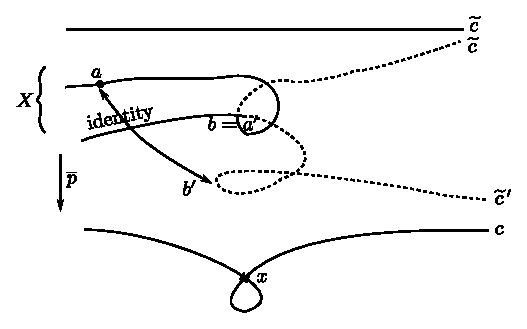
\includegraphics{fig1.eps}
\end{figure}

\item Let\pageoriginale $X$ and $S$ be irreducible algebraic varieties
  and suppose 
  that $S$ is normal and $f:X\to S$ a dominant morphism. Assume, in
  addition, that the function field $R(X)$ of $X$ is a finite
  extension of degree $n$ of the function field $R(S)$ of $S$. If
  $x\in X$ is such that the number of points in the fibre
  $f^{-1}(f(x))$ equals $n$, then it can be shown that $f$ is \'etale
  in a neighbourhood of $x$.  
\end{enumerate}

\section{}\label{chap3-sec3.3}%3.3
Our aim now is to give a necessary and sufficient condition for a
morphism to be unramified. 

\setcounter{subsection}{-1}
\subsection{Some algebraic preliminaries.}\label{chap3-sec3.3.0}%3.3.0

Let $A\xrightarrow{\varphi}B$ be a homomorphism of rings defining an
$A$-algebra structure on $B$. Then $\foprod{B}{B}{A}$ is an $A$-algebra
in a natural way and
\begin{align*}
& p_{1}:B\to \foprod{B}{B}{A}\text{ \ given by \ } b\mapsto b\otimes 1\\
& p_{2}:B\to \foprod{B}{B}{A}\text{ \ given by \ } b\mapsto 1\otimes b
\end{align*}
and $\mu:\foprod{B}{B}{A}\to B$ given by $b_{1}\otimes b_{2}\mapsto
b_{1}b_{2}$ are all $A$-algebra homomorphisms. We may make
$\foprod{B}{B}{A}$ a $B$-algebra through $p_{1}$ i.e. by defining
$b(b_{1}\otimes b_{2})=bb_{1}\otimes b_{2}$ and the kernel $I$ of
$\mu$ is then a $B$-module. Since we have $\mu\circ p_{1}=\Id.$ and
the equality $b_{1}\otimes b_{2}=(b_{1}b_{2}\otimes
1)-b_{1}(b_{2}\otimes 1-1\otimes b_{2})$ is follows that
$\foprod{B}{B}{A}=(\foprod{B}{1}{A})\oplus I$, as a $B$-module.

We\pageoriginale define the space $\Omega_{B/A}$ of $A$-differentials
of $B$ as the $B$-module $I/I^{2}$. We note that the $B$-module
structure on $\Omega_{B/A}=I/I^{2}$ is natural, in the sense that it
does not depend on whether we make $\foprod{B}{B}{A}$, a $B$-algebra
through $p_{1}$ or through $p_{2}$.

\section*{Some properties of $\Omega_{B/A}$}

\begin{enumerate}
\renewcommand{\labelenumi}{(\theenumi)}
\item The map $d:b\mapsto (1\otimes b-b\otimes 1)$ $\pmod{I^{2}}$ from
  $B$ to $\Omega_{B/A}$ is $A$-linear. Also, since
\begin{align*}
(1\otimes b_{1}b_{2}-b_{1}b_{2}\otimes 1) &= b_{1}(1\otimes
  b_{2}-b_{2}\otimes 1)+b_{2}(1\otimes b_{1}-b_{1}\otimes 1)\\
&= +(1\otimes b_{1}-b_{1}\otimes 1)(1\otimes b_{2}-b_{2}\otimes 1),
\end{align*}
we have: $d(b_{1}b_{2})=b_{1}db_{2}+b_{2}db_{1}\ \forall\ b_{1}$,
$b_{2}\in B$.

\item Since $I$ is generated as a $B$-module by elements of the form
  $(1\otimes b_{1}-b_{1}\otimes 1)$, it follows that $\Omega_{B/A}$ is
  generated by the elements $db$.

\item Let $W$ be the $B$-submodule of $\foprod{B}{B}{A}$, generated by
  elements of the form $(1\otimes bb'-b\otimes b'-b'\otimes b)$;
  $\Omega_{B/A}$ is then isomorphic to $(\foprod{B}{B}{A})/W$.

In fact,
\begin{align*}
\Omega_{B/A} &= I/I^{2}\cong (\foprod{B}{1}{A}\oplus
I)/(\foprod{B}{1}{A}\oplus I^{2})\\
&= (\foprod{B}{B}{A})/(\foprod{B}{1}{A}\oplus I^{2})
\end{align*}
and\pageoriginale clearly $W\supset \foprod{B}{1}{A}$; so $W=B\otimes
1\oplus (W\cap I)$.

On the other hand, we have
$$
(1\otimes bb'-b\otimes b'-b'\otimes b)=-bb'\otimes 1+(1\otimes
b-b\otimes 1)(1\otimes b'-b'\otimes 1)
$$
and hence: $W\subset \fprod{B}{1}{A}\oplus I^{2}$. Also clearly,
$I^{2}\subset W$. It follows that $W\cap I-I^{2}$,
$W=\foprod{B}{1}{A}\oplus I^{2}$ and $\Omega_{B/A}\cong
(\foprod{B}{B}{A})/W$.

\item If $V$ is any $B$-module and $D:B\to V$ any $A$-derivation of
  $B$ in $V$, then there is a $B$-linear map $H_{D}:\Omega_{B/A}\to V$
  such that
\[
\xymatrix{
B\ar[rr]^{D}\ar[dddr]_{d}  & & V\\
 &  \ar@/_1pc/@{-_{>}}[dlr]  & \\
 & &\\
 &  \Omega_{B/A}\ar[uuur]_{H_{D}} &
}
\]
In fact, $D$ defines an $A$-linear map $\foprod{B}{B}{A}\to V$ given by
$b_{1}\otimes b_{2}\mapsto b_{1}Db_{2}$. This is certainly $B$-linear
and is trivial on $W$. We then obtain a $B$-linear map
$H_{D}:\Omega_{B/A}\to V$ such that $H_{D}(db)=Db\ \forall\ b\in B$. Also
the correspondence $D\mapsto H_{D}$ is a $B$-isomorphism from the
$B$-module of $A$-derivations $B\to V$, onto the $B$-module
$\Hom_{B}\break (\Omega_{B/A},V)$. (This is the universal property of
$\Omega_{B/A}$). In particular, the $B$-module of $A$-derivations of
$B$ is isomorphic to $\Hom_{B}\break (\Omega_{B/A},B)$; and even more in
particular, if\pageoriginale $A=k$, $B=K$ are fields, we see that the
space of $k$-differentials $\Omega_{K/k}$ is the dual of the space of
$k$-derivations of $K$ and therefore is trivial if $K/_{k}$ is
separably algebraic. 

\item Consider a base-change $A\to A'$ and the extension of scalars
  $B'=\foprod{B}{A'}{A}$. From the universal property of the space of
  differentials, it follows that
$$
\Omega_{B'/A'}\simeq
\foprod{\Omega_{B/A}}{B'}{B}\foprod{\Omega_{B/A}}{A'}{A}. 
$$
\end{enumerate}

\subsection{The sheaf of differentials of a
  morphism.}\label{chap3-sec3.3.1}

~

Let $f:X\to S$ be a morphism. Our aim now is to define a sheaf
$\Omega_{X/S}$ on $X$. Assume, to start with, that $X=\Spec B$,
$S=\Spec A$; then $\Omega_{B/A}$ is a $B$-module in a natural way and
we define $\Omega_{X/S}=\widetilde{\Omega}_{B/A}$ on $X$. In the
general case, consider the diagonal $\Delta$ of $f$ in
$\fprod{X}{X}{S}$. Then $\Delta$ is a closed subscheme of an open
subscheme $U$ of $\fprod{X}{X}{S}$ and $X\to \Delta$ is an
isomorphism. Let $I_{X}$ be the sheaf of ideals of $\mathscr{O}_{U}$
defining $\Delta$. Then $I_{X/I^{2}_{X}}$ is a sheaf of
$\mathscr{O}_{U}$-modules whose support is contained in $\Delta$. By
means of the isomorphism $X\to \Delta$, we can lift this sheaf to a
sheaf of abelian groups on $X$. Clearly the lift is independent of the
choice of $U$. It remains to show that this sheaf is an
$\mathscr{O}_{X}$-Module. To do this, we can assume again that
$X\times S$ are affine and in this case, $I_{X}$ is the
sheaf\pageoriginale $\widetilde{I}$ on $\fprod{X}{X}{S}$ (where $I$ is
the ideal of $\foprod{B}{B}{A}$ defined in \ref{chap3-sec3.3.0}) and
therefore, our sheaf is $\widetilde{\Omega}_{B/A}$ considered above.

The $\mathscr{O}_{X}$-Module thus obtained will be called the {\em
  sheaf of differentials} of $f$ (or of $X$ over $S$) and will be
denoted $\Omega_{X/S}$. The stalk $\Omega_{x,X/S}$ of this sheaf at a
point $x\in X$ is canonically isomorphic to
$\Omega_{\mathscr{O}_{x}/\mathscr{O}_{f(x)}}$. This is seen either
from the universal property or by observing that the natural map
$\Omega_{x,X/S}\to \Omega_{\mathscr{O}_{x}/\mathscr{O}_{f(x)}}$ given
by
$$
\sum_{i}\frac{b_{i}}{s_{i}}db'_{i}\mapsto
\sum_{i}\frac{b_{i}}{s_{i}}d(b'_{i/1})\quad (\text{with } X=\Spec
B,b_{i},b'_{i},s_{i}\in B, s_{i}\not\in \underline{p}_{x}) 
$$
is an isomorphism.

Since, by assumptions, $S$ is locally noetherian and $f$ is of finite
type it is cler from the definition that $\Omega_{X/S}$ is coherent.

\setcounter{section}{3}
\setcounter{prop}{1}
\begin{prop}\label{chap3-prop3.3.2}
For a morphism $f:X\to S$ and a point $x\in X$ the following are equivalent:
\begin{itemize}
\item[\rm(i)] $f$ is unramified at $x$

\item[\rm(ii)] $\Omega_{x,X/S}=(0)$

\item[\rm(iii)] $\Delta:X\to \fprod{X}{X}{S}$ is an open immersion in a
  neighbourhood of $x$.
\end{itemize}
\end{prop}

\begin{proof}
We\pageoriginale may assume $X=\Spec B$, $S=\Spec A$.

\medskip
(i) $\Rightarrow$ (ii):~Consider the base change:
\[
\xymatrix@=1.2cm{
x\in X\ar[d] & X'=X\fprod{S}{\Spec k(s)}{S}\ar@{->}[l]\ar[d]\\
s=f(x)\in S & \Spec k(s)=S'\ar@{->}[l]
}
\]

If $x'\in X'$ is above $x$, then we have:
$\foprod{\Omega_{x,X/S}}{\mathscr{O}_{x'}}{\mathscr{O}_{x}}=\Omega_{x',X'/S'}$;
this follows from property (5) of \ref{chap3-sec3.3.0}; furthermore,%raghu
$\mathscr{O}_{x'}=\mathscr{O}_{x/\mathscr{M}_{s}\mathscr{O}_{x}}=k(x)$
since $f$ is unramified at $x$. Therefore
$\foprod{\Omega_{x,X/S}}{k(x)}{\mathscr{O}_{x}}=\Omega_{x',X'/S'}$ and
by Nakayama it suffices to show that the latter is (0). By the remark
made above, $\Omega_{x',X'/S'}=\Omega_{k(x)/k(s)}$ and this is zero as
$k(x)/k(s)$ is separably algebraic.

\medskip
(ii) $\Rightarrow$ (iii)

Let $z$ be the image of $x$ in $\fprod{X}{X}{S}$ under the diagonal
$\Delta:X\to \fprod{X}{X}{S}\cdot \Delta(X)$ is a closed subscheme of
an open subscheme $U$ of $\fprod{X}{X}{S}$, and is defined, therefore,
by a sheaf $I$ of $\mathscr{O}_{U}$-ideals. If $\Omega_{x,X/S}=(0)$,
then, we will have $I_{z}=I^{2}_{z}=\ldots$; hence\pageoriginale
$I_{z}=(0)$ (Krull's intersection theorem). However, $I$ is a sheaf of
ideals of finite type and so $I$ vanishes in a neighbourhood of $z$
i.e. to say $\Delta:X\to \fprod{X}{X}{S}$ is an open immersion in a
neighbourhood of $x\in X$.

\medskip
(iii) $\Rightarrow$ (i)

The question being local, we may assume that $\Delta:X\to
\fprod{X}{X}{S}$ is an open immersion everywhere. An open immersion
remains an open immersion under base-change, and since we only have to
look at the fibre over $f(x)$, for non-ramification at $x$, we may
take $X=\Spec A$, $S=\Spec k$, $k$ a field and $A$ a $k$-algebra of
finite type.

We are to show that $A=\bigoplus\limits_{\text{finite}}K_{i}$, where
$K_{i/k}$ are finite separable field extensions; for this, we have to
show that $A$ is artinian and, if $\overline{k}$ is the algebraic
closure of $k$, $\foprod{A}{\overline{k}}{k}$ is radical-free. It is
thus enough to show that
$\foprod{A}{\overline{k}}{k}=\bigoplus\limits_{\text{finite}}\overline{k}$. By
making the base-change $k\to \overline{k}$, we may assume $k$ is
algebraically closed.

Let $a\in X$ be any closed point of $X$. Since $k$ is algebraically
closed, $k(a)\simeq k$ and we have then
\begin{gather*}
X\xleftarrow[i]{\sim} \fprod{X}{\Spec}{\Spec k} k(a)=X\times
(a)\quad\text{(say).}\\
X\times (a)\quad\text{is canonically imbedded in } \fprod{X}{X}{S}
\end{gather*}
and let $\varphi$ be the composite of the morphisms:
$$
X\xrightarrow{i^{-1}}X\times (a)\hookrightarrow \fprod{X}{X}{S}. 
$$

Then\pageoriginale $\varphi^{-1}(\Delta)=(a)$ is open in $X$, since,
by assumption, $\Delta$ is open in $\fprod{X}{X}{S}$; i.e. any closed
point of $X$ is also open. But $X=\Spec A$ is quasi-compact and this
implies that $A$ has only finitely many maximal ideals. But $A$ is a
$k$-algebra of finite type and so the set of closed points of $X$ is
dense in $X$. It follows that $A$ is artinian and we may write
$A=\bigoplus\limits^{\dot{n}}_{i=1}A_{i}$ where the $A_{i}$ are
artinian local rings. We may then assume $A=A_{i}$; the open immersion
$\Delta:X\to \fprod{X}{X}{S}$ then gives an isomorphism
$\foprod{A}{A}{k}\to A$. This however means $A=k$.\hfill Q.E.D.
\end{proof}

\setcounter{subsection}{2}
\subsection{Some properties of \'etale morphisms.}\label{chap3-sec3.3.3}

\begin{itemize}
\item[(1)] An open immersion is \'etale.

\item[(2)] $f$, $g$ \'etale $\Rightarrow g\circ f$ \'etale.

\item[(3)] $f$ \'etale $\Rightarrow f_{(S')}$ \'etale for {\em any}
  base change $S'\to S$

({\em not necessarily of finite type}), $S'$, $S$ locally noetherian.

This follows from condition (iii) of Proposition \ref{chap3-prop3.3.2}, the
facts that an open immersion remains an open immersion and that a flat
morphism remains flat under base change.

\item[(4)] $f_{1}$, $f_{2}$ \'etale $\Rightarrow
  \fprod{f_{1}}{f_{2}}{S}$ \'etale. 


Follows from (2), (3) and the equality
$$
\fprod{f_{1}}{f_{2}}{S}=(\fprod{f_{1}}{I_{Y_{2}}}{S})\circ
(\fprod{I_{X_{1}}}{f_{2}}{S}). 
$$

\item[(5)] $g\circ f$\pageoriginale \'etale, $g$ unramified $\Rightarrow f$
  \'etale.

Let $f:X\to Y$ and $g:Y\to Z$. The question being local, we may assume
from (iii) Proposition \ref{chap3-prop3.3.2} that $\Delta=\Delta(Y):Y\to
\fprod{Y}{Y}{Z}$ is an open immersion, hence \'etale. By the
base-change $X\xrightarrow{f}{Y}$ we get $\Delta_{(X)}:X\to
\fprod{X}{Y}{Z}$ which again is \'etale by (3). The diagram:
\[
\xymatrix@R=.5cm@C=1cm{
X\ar[ddd]^{g\circ f} & & & \ar[lll] \fprod{X}{Y}{Z}\ar[ddd]^{p_{2}}\\
 & \ar@/^1pc/@{-_{>}}[dr] & & \\
 & & & \\
Z\ar@{<-}[rrr]_{g} & && Y
}
\]
shows that the second projection $p_{2}:\fprod{X}{Y}{Z}\to Y$ is given
by $(g\circ f)_{(Y)}$; so, again by (3), $p_{2}$ is also \'etale and
from (2) we obtain that $f=p_{2}\circ
\Delta_{(X)}:X\xrightarrow{\Delta_{(X)}}\fprod{X}{Y}{Z}\xrightarrow[p_{2}]{}Y$
is \'etale.

\item[(6)] $g\circ f$ \'etale, $f$ \'etale $\Rightarrow g$ \'etale.


The composite: $\mathscr{O}_{gf(x)}\Rightarrow\mathscr{O}_{f(x)}\to
\mathscr{O}_{x}$ is flat and $\mathscr{O}_{f(x)}\to \mathscr{O}_{x}$
is faithfully flat, and thus $\mathscr{O}_{gf(x)}\to
\mathscr{O}_{f(x)}$ is flat. It is clear that $k(f(x))/_{k(g\cdot
  f(x))}$ is a finite separable\pageoriginale extension. Finally
$\mathscr{M}_{f(x)}\mathscr{O}_{x}=\mathscr{M}_{x}$ and
$\mathscr{M}_{g\cdot
  f(x)}\mathscr{O}_{x}=\mathscr{M}_{x}=(\mathscr{M}_{g\cdot
  f(x)}\mathscr{O}_{f(x)})\mathscr{O}_{x}$; since
$\mathscr{O}_{f(x)}\to \mathscr{O}_{x}$ is faithfully flat, it follows
that $\mathscr{M}_{g\cdot f(x)}\mathscr{O}_{f(x)}=\mathscr{M}_{f(x)}$.

\item[(7)] An \'etale morphism is an open map.
\end{itemize}

In fact, we prove more generally:


\setcounter{prop}{3}
\begin{prop}\label{chap3-prop3.3.4}
A flat morphism is an open map.
\end{prop}

The proposition will follow as a consequence from the lemmas below. We
first make the

\begin{defi*}
A subset $E$ of a noetherian topological space $X$ is said to be {\em
  constructible} if $E$ is a finite union of locally closed sets in $X$.
\end{defi*}

\setcounter{lemma}{4}
\begin{lemma}\label{chap3-lem3.3.5}
Let $X$ be a noetherian topological space and $E$ any set in
$X$. Then, $E$ is constructible $\Leftrightarrow$ for every
irreducible closed set $Y$ of $X$, $E\cap Y$ is either non-dense in
$Y$ or contains an open set of $Y$.
\end{lemma}

\begin{proof}
$\Rightarrow:$ Suppose $E=\bigcup\limits^{n}_{i=1}(O_{i}\cap F_{i})$,
  $O_{i}$ open, $F_{i}$ closed in $X$. Then $\overline{E\cap Y}\cap
  Y\subset \bigcup\limits^{n}_{i=1}(F_{i}\cap Y)$ for any closed
  $Y\subset X$; if $Y$ is irreducible with $E\cap Y$ dense in $Y$,
  this means $Y\subset F_{i}\cap Y$ for some $i$, i.e., $F_{i}\supset
  Y$; then $Y\cap E\supset (O_{i}\cap Y)$ open in $Y$.

$\Leftarrow :$\pageoriginale We shall prove this by noetherian
  induction. Let $\mathscr{E}$ be the set of all closed sets $F$ in
  $X$ such that $E\cap F$ is not constructible. If $\mathscr{E}\neq
  \emptyset$ choose a minimal $F_{0}\in \mathscr{E}$. By replacing $X$
  by $F_{0}$, we may assume that for every closed set $F$ properly
  contained in $X$, $E\cap F$ is constructible. If $X$ is reducible,
  say $X=X_{1}\cup X_{2}$, $X_{1}$, $X_{2}$ both proper subsets of $X$
  and closed, then $E\cap X_{1}$, $E\cap X_{2}$ are both constructible
  and hence so is $E=(E\cap X_{1})\cup (E\cap X_{2})$. If $X$ is
  irreducible, either
\begin{itemize}
\item[(i)] $\overline{E}\neq X$ and so $E=E\cap \overline{E}$ is
  constructible or

\item[(ii)] $E\supset U\neq \emptyset$, $U$ open, so that $E=U\cup
  (E\cap (X-U))$ is still constructible. This contradiction shows that
  $\mathscr{E}=\emptyset$.\hfill Q.E.D.
\end{itemize}
\end{proof}

\begin{lemma}\label{chap3-lem3.3.6}
Let $S$ be a noetherian prescheme and $f:X\to S$ a morphism. Then the
image, under $f$, of any constructible set is constructible.
\end{lemma}

\begin{proof}
Using the preceding lemma, the fact that $S$ is noetherian and by
passing to subschemes, irreducible components and so on, we are
readily reduced to proving the following assertion: if $X$, $S$ are
both affine, reduced, irreducible and noetherian and if $f:X\to S$ is
a morphism of finite type such that $\overline{f(X)}=S$, then $f(X)$
contains an open subset of $S$. 

If\pageoriginale $X=\Spec B$, $S=\Spec A$, our assumptions mean that
$A$, $B$ are noetherian integral domains and the ring-homomorphism
$A\to B$ defining $f$ is then easily checked to be an injection. The
lemma will then follow from the following purely algebraic result. 
\end{proof}

\begin{lemma}\label{chap3-lem3.3.7}
Let $A$ be an integral domain and $B=A[x_{1},\ldots,x_{n}]$ an
integral $A$-algebra containing $A$. Then there exists a $g\in A$ such
that for every prime ideal $\underline{p}$ of $A$ with $g\not\in
\underline{p}$, there is a prime ideal $\mathscr{P}$ of $B$ such that
$\mathscr{P}\cap A=\underline{p}$.
\end{lemma}

\begin{proof}
Choose a transcendence base $X_{1},\ldots,X_{k}$ of $B/A$. Then the
extension $B=A[x_{1},\ldots,x_{n}]$ is algebraic over
$A'=A[X_{1},\ldots,X_{k}]$. By writing down the minimal polynomials of
the $x_{i}$ over $A'$ and by dividing out these polynomials by a
suitably chosen $g\in A$, $g\neq 0$, we can make the $x_{i}$ integral
over $A'\left[\frac{1}{g}\right]$. Consider now the tower of
extensions.
\[
\xymatrix{
B\left[\frac{1}{g}\right]\ar@{-}[d]\\
A'\left[\frac{1}{g}\right]\ar@{-}[d]\\
A\left[\frac{1}{g}\right]\ar@{-}[d]\\
A
}
\]

If $\underline{p}$ is a prime ideal of $A$ such that $g\not\in
\underline{p}$ then there is a prime $\underline{p}'$ of
$A\left[\frac{1}{g}\right]$ lying over $\underline{p}$. The prime
ideal $\ub{p}'+(X_{1},\ldots,X_{k})$ of $A'\left[\frac{1}{g}\right]$
lies over $\ub{p}$. Now $\left[\frac{1}{g}\right]$ is a finite
extension of $A'\left[\frac{1}{g}\right]$
and by Cohen-Seidenberg, $\exists$ a prime ideal $\mathscr{P}'$ of
$B\left[\frac{1}{g}\right]$ lying over $\ub{p}$. The restriction
$\mathscr{P}$ of $\mathscr{P}'$ to $B$ then sits over $\ub{p}$.\hfill Q.E.D.
\end{proof}

\begin{lemma}\label{chap3-lem3.3.8}
Let\pageoriginale $f:X\to S$ be a morphism (of finite type) and
$T\subset X$ be an open neighbourhood of a point $x\in X$. Assume that
for every $s_{1}\in S$ such that $f(x)\in \overline{(s_{1})}$, there
is a $t_{1}\in T$ such that $f(t_{1})=s_{1}$. Then $f(T)$ is a
neighbourhood of $f(x)$. 
\end{lemma}


\begin{proof}
Since the question is local, we may assume $S$ noetherian and then by
lemma \ref{chap3-lem3.3.6} it follows that $f(T)$ is constructible. We may
then write $f(T)=\bigcup\limits_{i=1}(O_{i}\cap F_{i})$; and by
choosing only those $i$, for which $f(x)\in O_{i}$, we may say that
$f(T)$ is closed in a neighbourhood of $f(x)$. The hypotheses show
that $f(T)$ is also dense in a neighbourhood of $f(x)$. It follows
that $f(T)$ is itself a neighbourhood of $f(x)$.\hfill Q.E.D.
\end{proof}

\medskip
\noindent
{\bf Proof of Proposition \ref{chap3-prop3.3.4}.}
\smallskip

In view of the lemma \ref{chap3-lem3.3.8}, it suffices to show that if
$U\subset X$ is an open neighbourhood of $x\in X$, $f(U)$ contains all
generisations of $f(x)$. The generisations of $f(x)$ are the points of
$\Spec \mathscr{O}_{f(x)}$ and those of $x$ are points of $\Spec
\mathscr{O}_{x}$. But $\mathscr{O}_{x}$ is
$\mathscr{O}_{f(x)}$-faithfully flat and then it is well-known for any
prime ideal $\ub{p}$ of $\mathscr{O}_{f(x)}$, there is a prime-ideal
$\mathscr{P}$ of $\mathscr{O}_{x}$ contracting to $\ub{p}$. $U$ being
open we have $\Spec \mathscr{O}_{x}\subset U$. Hence $\Spec
\mathscr{O}_{f(x)}\subset f(U)$ (cf. Bourbaki, Alg. Comm. Ch. II,
\S\ 2, n$^\circ$5, Cor. 4 to Proposition 11).\hfill Q.E.D.


\section{}\label{chap3-sec3.4}

A\pageoriginale morphism $f:S'\to S$ is said to be an {\em effective
  epimorphism} if the sequence
\[
\xymatrix{
S''=\fprod{S'}{S'}{S} \ar@<.5ex>[r]^-{p_{1}} \ar@<-.5ex>[r]_-{p_{2}} &
S'\ar[r]^-{f} & S\text{\quad is exact}
}
\]
i.e., if the sequence $\xymatrix{
\Hom (S,Y)\ar[r] & \Hom(S',Y) \ar@<.5ex>[r]^-{p_{1}^{\ast}}
\ar@<-.5ex>[r]_-{p_{2}^{\ast}} & \Hom(S'',Y)}$ is exact, as a sequence
of sets, $\forall Y$.

(We say that a sequence of sets $\xymatrix{E_{1}\ar[r]^{h_{1}} &
  E_{2}\ar@<.5ex>[r]^{h_{2}}\ar@<-.5ex>[r]_{h'_{2}}& E_{3}}$ is exact
if $h_{1}$ is an injection and $h_{1}(E_{1})=\{x\in
E_{2}:h_{2}(x)=h'_{2}(x)\}$). 

A morphism $f:S'\to S$ is {\em faithfully flat} if it is flat and
surjective. Our aim now is to show that any such morphism is an
effective epimorphism.

\subsection{Some algebraic preliminaries; the Amitsur
  complex.}\label{chap3-sec3.4.1} 

A homomorphism of rings $f:A\to A'$ defines a sequence:
\[
\xymatrix{
A\ar[r]^{f} & A'\ar@<.2em>[r]^-{p_{1}}\ar@<-.2em>[r]_-{p_{2}} &
\foprod{A'}{A'}{A}=A''\ar@<1em>[r]^-{p_{21}}\ar[r]^-{p_{32}}\ar@<-.5em>[r]_-{p_{31}}  
&
\foprod{A'}{\foprod{A'}{A'}{A}}{A}=A'''
\ar@<.9em>[r]\ar@<.5em>[r]\ar[r]\ar@<-.5em>[r]  &
}
\]
where $p_{1}(a')=a'\otimes 1$; $p_{2}(a')=1\otimes a'$,
$p_{21}(a'\otimes b')=a'\otimes b'\otimes 1$; $p_{31}(a'\otimes
b')=a'\otimes 1\otimes b'$; $p_{32}(a'\otimes b')=1\otimes a'\otimes
b'$ and so on.

We\pageoriginale may then define homomorphisms of $A$-modules:
\begin{align*}
\partial_{0} &= p_{1}-p_{2}\\
\partial_{1} &= p_{21}-p_{31}+p_{32}\\
\partial_{2} &= p_{321}-p_{421}+p_{431}-p_{432}\ldots
\end{align*}
and so on. One then checks that $\partial_{i+1}\partial_{i}=0\forall
i$; we thus get an augmented cochain complex:
$$
A\xrightarrow[f]{}A'\xrightarrow{\partial_{0}}A''\xrightarrow{\partial_{1}}A'''\xrightarrow{\partial_{2}}A''''\xrightarrow{\partial_{3}}\ldots .
$$

This complex is called the {\em Amitsur complex} $A'/A$.

\setcounter{subsection}{1}
\begin{sublemma}\label{chap3-lem3.4.1.1}
If $A\xrightarrow{f}A'$ is faithfully flat, then
\begin{itemize}
\item[\rm(i)] $A\xrightarrow{\sim}H^{0}(A'/A)$

\item[\rm(ii)] $H^{q}(A'/A)=(0)\forall q>0$.
\end{itemize}
\end{sublemma}

\begin{proof}
Suppose $B$ is any faithfully flat $A$-algebra.

Consider then the complex
$$
B'/B\equiv \foprod{B}{(A'/A)}{A}\equiv B\xrightarrow[1\otimes
  f]{}B'=\foprod{B}{A'}{A}\xrightarrow{1\otimes
  \partial_{0}}B''=\foprod{B'}{B'}{B}=\foprod{B}{A''}{A}\to 
$$

Since\pageoriginale $B$ is $A$-faithfully flat, it is enough to prove
that $H^{0}(B'/B)\xleftarrow{\sim}B$ and $H^{q}(B'/B)=(0)\forall
q>0$. As a particular choice we may take $B=A'$. Then the homomorphism
$A'\xrightarrow{f'=1\otimes f}\foprod{A'}{A'}{A}=A''$ admits a
section, i.e., $\exists \sigma :A''\to A'$ such that
$\sigma\circ f'=1_{A'}$, namely, the homomorphism: $a'\otimes b'\mapsto
a'b'$.

We may thus assume, without any loss of generality that the
homomorphism $A\xrightarrow{f}A'$ admits a section $\sigma:A'\to A$
such that $\sigma\circ f=1_{A}$:
\[
\xymatrix@R=0pt@C=1.5cm{
A\ar[r]^{f} & A'\ar[r]^{\partial_{0}} & A''\ar[r]^{\partial_{1}} &
A'''\ar[r]^{\partial_{2}}\ldots &.\\
 & \ar@/^1.5pc/[l]_{\sigma} &  
}
\]

We construct now a homotopy operator in this complex, as follows:
\[
\xymatrix{
A\ar[r]^{f}\ar[dr]_{1_{A}} &
A'\ar@<.2em>[r]^-{p_{1}}\ar@<-.2em>[r]_-{p_{2}}\ar[d]^{\sigma} &
\foprod{A'}{A'}{A}=A''\ar[d]^-{1\otimes\sigma} 
\ar@<.4em>[r]_-{p_{32}}\ar@<.8em>[r]^-{p_{21}}\ar@<-.7em>[r]_-{p_{31}} &
\foprod{A'}{\foprod{A'}{A'}{A}}{A}=A'''\ar[d]^{1\otimes 1\otimes
  \sigma} \ar@<.7em>[r]\ar@<.3em>[r]\ar@<-.05em>[r]\ar@<-.45em>[r] & \\
& A\ar[r]^-{f} & \foprod{A'}{A}{A}\xrightarrow{\sim}A'
\ar@<.2em>[r]^-{p_{1}}\ar@<-.2em>[r]_-{p_{2}} &
\foprod{A'}{\foprod{A'}{A}{A}}{A}\xrightarrow{\sim}A'' 
\ar[r]\ar@<.4em>[r]\ar@<-.4em>[r] & 
}
\]

\begin{itemize}
\item[(i)] $H^{0}(A'/A)=\ker \partial_{0}\xleftarrow{\sim}A$.

Let\pageoriginale $a'\in A'$ be such that
$p_{1}(a')=p_{2}(a')$. Applying $1\otimes 
\sigma$ we get $(1\otimes\sigma)(a'\otimes
1)=(1\otimes\sigma)(1\otimes a')$ i.e. $a'\otimes 1=1\otimes
\sigma(a')$ in $\foprod{A'}{A}{A}$. Under the canonical identification
$\foprod{A'}{A}{A}\xrightarrow{\sim}A'$, this means that
$$
a'=f(\sigma(a'))\quad\text{i.e.}\quad a'\in f(A).
$$
On the other hand, $f(A)\subset \ker \partial_{0}$ and $f$ being
faithfully flat, is injective. It follows that $\underline{\ker
  \partial_{0}\xleftarrow{\sim}A}$. 

\item[(ii)] By using the homotopy operator, one can show that
  $H^{q}(A'/A)=(0)\forall q>0$; the proof is omitted. (We do not need it).
\end{itemize}
\end{proof}

\subsection{}\label{chap3-sec3.4.2}

\setcounter{subsubsection}{2}
\begin{subprop}\label{chap3-prop3.4.2.1}
A faithfully flat morphism is also an effective epimorphism.
\end{subprop}

\begin{proof}
{\bf Case (a). {\boldmath$S'=\Spec A'$, $S=\Spec A$} are affine.}

From local algebra, it follows that the ring homomorphism
$A\xrightarrow{\varphi}A'$ defining $f:S'\to S$, is also faithfully
flat. We have to show that, for any $Y$, the sequence
\begin{equation*}
\Hom(S,Y)\to \Hom(S',Y)\rightrightarrows \Hom
(\fprod{S'}{S'}{S},Y)\text{\  is exact in } \calEns.\tag{*}
\end{equation*}

\begin{itemize}
\item[(i)] Suppose $Y=\Spec B$ is affine.

Then\pageoriginale the sequence (*) is equivalent to a sequence:
\begin{equation*}
\Hom(B,Z)\to \Hom(B,A')\rightrightarrows
\Hom(B,\foprod{A'}{A'}{A}).\tag*{$(*)'$} 
\end{equation*}

The exactness of this sequence $(\ast)'$ now follows from assertion
(i) of lemma \ref{chap3-lem3.4.1.1}.


\item[(ii)] Let $Y$ be arbitrary.

Let $\varphi_{1}:S\to Y$, $\varphi_{2}:S\to Y$ be two morphisms such
that $\varphi_{1}\circ f=\varphi_{2}\circ f$. Since $f$ is a
surjection, it is clear that $\varphi_{1}(s)=\varphi_{2}(s)\forall
s\in S$.

Choose a point $s\in S$ and a point $s'\in S'$ with $f(s')=s$; let
$y=\varphi_{1}(s)=\varphi_{2}(s)\in Y$. Choose an affine open
neighbourhood $\Spec B$ of $y\in Y$ and an element $\theta\in A$ such
that $s\in \Spec A_{\theta}$ and $\varphi_{1}(\Spec A_{\theta})\subset
\Spec B$, $\varphi_{2}(\Spec A_{\theta})\subset\Spec B$.

Set $\theta^{1}=\varphi(\theta)\in A'$. Then $s'\in \Spec
A'_{\theta'}$, and $f(\Spec A'_{\theta'})\subseteq \Spec A_{\theta}$;
and by (i) it follows that $\varphi_{1}$ and $\varphi_{2}$, when
restricted to $\Spec A_{\theta}$, define the same morphism of
preschemes. Since $s\in S$ was arbitrary, this proves that
$\Hom(S,Y)\to \Hom(S',Y)$ is injective.
\end{itemize}

Now, suppose that $\varphi':S'\to Y$ is a morphism such that in\pageoriginale
\[
\xymatrix{
S''=\fprod{S'}{S'}{S}\ar@<.2em>[r]^-{p_{1}}\ar@<-.2em>[r]_-{p_{2}} &
S^{1}\ar[dr]_{\varphi'}\ar[r]^{f} & S\\
& &  Y.
}
\]

We have $\varphi'\circ p_{2}=\varphi'\circ p_{1}$. We want to find a
morphism $\psi:S\to Y$ such that $\varphi'=\psi\circ f$.

In view of the injectivity established above, it is enough to define
$\psi$ locally. Let $s\in S$ and $s'\in S'$ with $f(s')=s$. Choose an
affine open neighbourhood $V$ of $\varphi'(s')$ in $Y$. Then the open
neighbourhood ${\varphi'}^{-1}(V)$ of $s'$ in $S'$ is saturated under
$f:$ in fact, let $x_{1}\in {\varphi'}^{-1}(V)$ and $x_{2}\in S'$ such
that $f(x_{1})=f(x_{2})$. Then, there is an $s''\in
S''=\fprod{S'}{S'}{S}$ such that $p_{1}(s'')=x_{1}$ and
$p_{2}(s'')=x_{2}$; so
$$
\varphi'(x_{1})=\varphi'\circ p_{1}(s'')=\varphi'\circ
p_{2}(s'')=\varphi'(x_{2})\quad\text{and}\quad x_{2}\in {\varphi'}^{-1}(V).
$$

Now, $f$ is flat and hence an open map (Prop. (\ref{chap3-prop3.3.4})) and
so\break $f({\varphi'}^{-1}(V))$ is an open neighbourhood of $s\in
S$. Choose an element $\theta\in A$ such that $s\in \Spec
A_{\theta}\subset f({\varphi'}^{-1}(V))$; if
$\theta^{1}=\varphi(\theta)\in A'$ then $f(\Spec A'_{\theta'})=\Spec
A_{\theta}$, and $\Spec A'_{\theta'}=f^{-1}(\Spec A_{\theta})\subset
{\varphi'}^{-1}(V)$ since ${\varphi'}^{-1}(V)$ is saturated under $f$.

We\pageoriginale then have a diagram
\[
\xymatrix@R=1.5cm{
 &
  \Spec(\fprod{A'_{\theta'}}{A'_{\theta'}}{A_{\theta}})\ar@<.6em>[d]_{p_{2}}\ar@<-.6em>_{p_{1}}[d]\\
& \Spec A'_{\theta'}\ar[dl]^{\varphi'}\ar[d]^{f}\\
V & \Spec A_{\theta}=f(\Spec A'_{\theta'})
}
\]

The problem of defining $\psi:\Spec A_{\theta}\to V$ is now a purely
affine problem and we are back to (i).

\medskip
{\bf Case (b). The general case.}
\smallskip

Without loss of generality, we may assume $S$ affine. Since $f$ is a
morphism of finite type, there is a finite affine open covering
$(S'_{\alpha})^{n}_{\alpha=1}$ of $S'$. Consider the disjoint union
$S^{\ast}=\coprod^{n}_{\alpha=1}S'_{\alpha}$. $S^{\ast}$ is affine and
the morphism $S^{\ast}\to S$ defined in the obvious way is again
faithfuly flat. Let $Y$ be an arbitrary prescheme and $F$ be the
(contravariant) functor $X\mapsto \Hom(X,Y)$. We have a commutative
diagram:
\[
\xymatrix@R=1.5cm{
F(S)\ar@{<->}[d]|\hole^{\kern -.5cm identity} \ar[r] & F(S')\ar@<.2em>[r]\ar@<-.2em>[r]\ar[d] &
F(S'')\ar[d]\\
F(S) \ar[r] & F(S^{\ast})\ar@<.2em>[r]\ar@<-.2em>[r] &
F(\fprod{S^{\ast}}{S^{\ast}}{S}) 
}
\] 

The\pageoriginale lower sequence is exact by case (a); the first
vertical map is the identity and the second vertical map is clearly
injective. Usual diagram - chasing shows that the upper sequence is
also exact.\hfill Q.E.D.
\end{proof}

\section{\'Etale coverings}\label{chap3-sec3.5}

\begin{defi*}
A morphism of preschemes, $f:X\to S$, is said to be {\em finite} if,
for every affine open $U\subset S$, $f^{-1}(U)$ is also affine and the
ring $\Gamma(f^{-1}(U),\mathscr{O}_{X})$ is a
$\Gamma(U,\mathscr{O}_{S})$-{\em module} of finite type.
\end{defi*}

It is again enough to check the conditions for an affine open cover of
$S$.
\begin{enumerate}
\renewcommand{\labelenumi}{(\theenumi)}
\item If $S$ is locally noetherian and $f:X\to S$ is a finite
  morphism, $f_{\ast}(\mathscr{O}_{X})$ is a coherent
  $\mathscr{O}_{S}$-Module.

\item A finite morphism remains finite under a base-change.

In particular, if $f:X\to S$ is finite and $s\in S$ any point, the
morphism $f_{\Spec k(s)}:\fprod{X}{k(s)}{S}\to k(s)$ is finite and
this means that the fibre $f^{-1}(s)$ is finite, discrete.

\item A finite morphism is proper.

In face, a finite morphism is affine and is hence separated; it
remains finite under any base-change and so it is enough to show that
a finite morphism is closed.

By\pageoriginale obvious reductions, we may take $X$, $S$ affine
reduced and $\overline{f(X)}=S$. If $X=\Spec B$ and $S=\Spec A$, the
corresponding homomorphism $A\to B$ is an injection and $B$ is a
finite $A$-module. Cohen-Seidenberg then shows that $f(X)=S$.

\item The following result holds:
\end{enumerate}

\begin{lemma}[Chevalley]\label{chap3-lem3.5.1}
Let $S$ be (as always) locally noetherian and $f:X\to S$ a morphism of
preschemes. Then the following conditions are equivalent:
\begin{itemize}
\item[\rm(a)] $f$ is finite

\item[\rm(b)] $f$ is proper and affine

\item[\rm(c)] $f$ is proper and $f^{-1}(s)$ is {\em finite} $\forall s\in
  S$.
\end{itemize}
\end{lemma}

(For a proof see EGA Ch.III (a) Proposition (4.4.2)).

\begin{defi*}
A morphism $f:X\to S$ is said to be an {\em \'etale covering} if it is
both \'etale and finite.
\end{defi*}

Let $X\xrightarrow{f}S$ be an \'etale covering. Then
$f_{\ast}(\mathscr{O}_{X})$ is a locally free
$\mathscr{O}_{S}$-Algebra of finite rank. For any $s\in S$, the fibre
$\foprod{f_{\ast}(\mathscr{O}_{X})}{k(s)}{S}$ is a finite direct sum
$\sum\limits^{n_{s}}_{i=1}K_{i}$ of finite separable field extensions
$K_{i}$ of $k(s)$. The rank of $f_{\ast}(\mathscr{O}_{X})$ at $s\in S$
is then given by $\sum\limits^{n_{s}}_{i=1}[K_{i}:k(s)]$ which equals
the number of geometric points in the fibre $f^{-1}(s)$. This is
constant in each connected component of $S$; if $S$ is connected, this
constant rank is\pageoriginale called the {\em degree} or the {\em
  rank} of the covering $f$. In this case, if this rank equals 1, then
$f$ is an isomorphism.

\begin{note*}
For \'etale coverings we have properties similar to (2), (3) (with
$S'\to S$ {\em not} necessarily of finite type) (4), (5) and (6) from
\ref{chap3-sec3.3.3}; this follows immediately from \ref{chap3-sec3.3.3} and
properties of coverings.
\end{note*}

\medskip
\noindent
{\bf A word of caution:}
\smallskip

This concept of an ``\'etale covering'' (French: rev\^etement
\'etale)\break 
should {\em not} be confused with the concept of a ``covering in the
\'etale topology'' (French: famille couvrante). The latter concept is
        {\em not} treated in this course. We also note that an \'etale
        covering, as defined here, is not necessarily surjective if
        $S$ is not connected.



